\documentclass[12pt]{article}
\usepackage{fancyhdr}
\usepackage{lastpage}
\usepackage{amsthm}
\usepackage[sorting=none]{biblatex}
\usepackage{hyperref}
\usepackage{amsmath}
\usepackage{amsfonts}
\usepackage{siunitx}
\usepackage{mathabx}
\usepackage[inkscapelatex=false]{svg}
\usepackage{footnote}
\usepackage{tablefootnote}
\usepackage{makecell}
\usepackage[letterpaper, left=2cm,right=2cm,top=3cm,bottom=2cm]{geometry}
\usepackage{longtable}
\usepackage{multirow}
\usepackage{array}
\usepackage{verbatim}
\usepackage{minted}
\usepackage{booktabs}
\usepackage{algorithm}
\usepackage{algpseudocode}
\usepackage{subcaption}
\usepackage{graphicx}
\usepackage{subfigure}
\usepackage[toc,page]{appendix}
\usepackage[version=4]{mhchem}
\usepackage{setspace}
\usepackage{placeins}
\usepackage[]{pdfpages}
\usepackage{wrapfig}

\renewcommand{\maketitle}{
    \begin{center}{
        
    {\fontsize{10pt}{14pt}\selectfont Team Control Number}\\[0.5em]
    
    {\fontsize{24pt}{14pt}\selectfont \textcolor{red}{\textbf{13879}}}\\[0.4em]
    
    {\fontsize{10pt}{14pt}\selectfont Problem Chosen}\\[0.5em]
    
    {\fontsize{24pt}{14pt}\selectfont \textcolor{red}{\textbf{A}}}\\[0.5em]

    {\fontsize{14pt}{14pt}\selectfont \textbf{2023}}\\[-0.2em]

    {\fontsize{10pt}{14pt}\selectfont \textbf{HiMCM}}\\[-0.2em]

    {\fontsize{10pt}{14pt}\selectfont \textbf{Summary Sheet}}\\[4em]
    
    }\end{center}
    \hrule
    \normalsize
}
% new command
\renewenvironment{abstract}{\maketitle}{\newpage\setlength{\parskip}{0em}\tableofcontents\setlength{\parskip}{0.5em}\newpage}
% format
\pagestyle{fancy}
\fancyhf{}
\rhead{Page \thepage\ of \pageref*{LastPage}}
\lhead{Team \#13879}
\setlength{\parindent}{0em}
\setlength{\parskip}{1em}

% citation
\addbibresource{citation.bib}
\hypersetup{
  colorlinks=true,
  urlcolor=blue,
  linkcolor=red,
  citecolor=red
}
\begin{document}
\begin{abstract}
    Dandelions are known as constructive medical raw materials, which also support the economy. However, some regard dandelions as invasive species due to their ability to endure the harsh environment and fast speed of propagation. Based on that circumstance, this paper delves into the investigation of dandelion population prediction as well as its impact factors on the risk index.

In the first section, we develop a differential equation model to describe the behavior of the dandelion population. We first divide the population into two main groups: seeds and puffballs. Considering their respective properties, we separate them into two different differential equations. In the next step, we gave each of the parameters in the differential equation a concise and reasonable formula. In addition, we have taken resource competitionabs into consideration, which further completely describes their behaviors. By evaluating growth rate, reproduction rate, death rate as well and resource competition, we finally derived around $160$ dandelions in a one-hectare area.

In the next section, we used the Cellular Automaton model to simulate the behavior of dandelions from a concrete perspective. We divided the field into a lattice made up of tons of square cells, with a side length of $\SI{0.01}{m}$. In the lattices, each cell either contains a dandelion or not. For those containing a dandelion, the dandelion will interact with the resource level of cells around it. The interaction can better describe the individuality of the dandelions, the long-term interaction, the regional differences, and the continuity of the life span. Via doing this, the result can generate a vivid visualization of the field, and give us more information about the periodic behaviors and inter-plant influences.

In response to question 2, we construct an evaluation model to assess the invasiveness of dandelions. By introducing a list of differential equations, we successfully analyze the interaction between two species. Instead of solely focusing on the contributions of different factors to the impact factor, we take an indirect step, concentrating on the parameters in the differential equations. Then we incorporate the AHP model to further outline the importance of various factors to the parameters, and then to the impact factor. With that thought, we ultimately conclude that dandelions should be considered an invasive species, as well as Pueraria montana and tumbleweeds, the two publicly acknowledged invasive species.
    
    \textbf{Keywords:} Dandelion, Invasion Species, Differential equation, Cellular Automaton, AHP
\end{abstract}
% Section 1

\newpage

\section{Introduction}
\subsection{Background}
As technology for transporting becomes increasingly facilitated, species could travel from region to region more effortlessly, leading to the appearance and development of invasive plants. Invasive species predate, compete, parasite, or spread disease among native species, leading to a malignant influence on the ecosystem and local economy \cite{barbier_implementing_2013}. In 2023, 40 percent of native species in North America were affected and threatened by invasive plants, and 35 billion was spent on controlling the number of invasive species in 2009 \cite{chornesky_threat_2003}. Among all the invasive species, plants’ spreading mode is the easiest to simplify, which can be applied in researching the spread mode of others. 

Among all the spreading modes for plants, wind propagation is the fundamental one. Dandelion is one of the most famous plants spread by wind. Dandelions will experience the seed phase, flower phase, and Cypselae. In the seed phase and flower phase, Dandelions would sprout and bloom yellow flowers, which might be affected by temperature, soil fertility, elevation, etc. Cypselae means the feathery bristles acting like parachutes to assist seeds in spreading further \cite{lagidze_dandelion_2022}. During the process, the wind would carry a feather-like process with seeds to areas around, and the propagation process might be affected by humidity, wind conditions, etc. In our model, we aimed to find simple and accurate arithmetic to expose Dandelions’ spreading model, considering the competitive rate, Mortality caused by temperature, humidity, soil fertility as well as extreme weather, and growth rate. The model may assist people in finding out the spreading mode of invasive plants and then other invasive species. By preventing the spread of invasive species, ecology would be protected and less capital would be devoted.

\subsection{Problem Restatement}
In our model for the seed’s spreading mode for dandelions, we will consider natural factors that alter the reproduction rate and growth rate for dandelions. In consequence, we aim to inspire preventing the spread of invasive species, protecting the ecosystems, and saving capital.
\begin{itemize}
    \item  %point 1
    First of all, a model showing the propagation of a dandelion ready for spreading seeds that approaches an open one-hectare land will be constructed. The model will be available for forecasting the spread of dandelions in the first, second, third, sixth, and twelfth months, considering influencing factors like climate, temperature, humidity, etc. 
    \item %point 2
    Moreover, dandelions have played a role in the medical industry and food industry, some plantations still regard them as harmful weeds. Mentioning the complicated relationship between human beings and dandelions and our aim in helping with invasive species, the impact factor for dandelions will be calculated and tested by using the result above. After making sure the model works for dandelions, the impact factor of two more plants that are considered invasive in local regions would be computed.
\end{itemize}% 

\subsection{Variables \& Constants}
In this paper, we have made up an imaginary unit ``Resource Unit" for convenience. $1$ Resource Unit is equal to the resource accumulated by $1$ Square Meter of land in $1$ Day.
\begin{table}[H]
\centering
\caption{Variables used in the paper and explanations}
\label{variables}
\begin{tabular}{ccc}
    \toprule[2pt]
    Notation & Dimension & Explanation \\
    \midrule

    $N$ & \# & Total number of dandelions \\
    $S$ & \# & Number of dandelions in seed stage \\
    $P$ & \# & Number of dandelions in puffball stage \\
    $t$ & Day & Time \\
    $t_i$ & Day & Time since dandelion $i$'s seeding \\
    $\mu_r$ & per Day & Reproduction rate \\
    $\mu_g$ & per Day & Growth rate \\
    $\mu_{m,s}$ & per Day & Mortality of dandelion seeds \\
    $\mu_{m,p}$ & per Day & Mortality of dandelion puffballs \\
    $R_{(x,y)}$ & Resource Unit & Resource level at $(x,y)$ \\ %parameter
    $R_{t_i}$ & Resource Unit per \# & Resource absorbed on day $t_i$ \\
    $R_{\text{cri},t_i}$ & Resource Unit per \# & Critical resource required on day $t_i$ \\
    $R_d$ & Resource Unit per \# & The resource contained in a dead dandelion \\
    $S_{\text{eq}}$ & \# & Equivalent amount of seeds \\
    $P_{\text{eq}}$ & \# & Equivalent amount of puffballs \\
    $\alpha_{n,s}$ & No Unit & Mortality by nutrition lack for seeds\\
    $\alpha_{n,p}$ & No Unit & Mortality by nutrition lack for puffballs\\
    $\alpha$ & No Unit & Mortality by other environmental factors\\ %parameter
    $l$ & Meter & Side length of the lattice \\ %parameter
    $r_{t_i}$ & Meter & Radius of dandelions' root on day $t_i$ \\
    $\lambda_{t_i}$ & per Day per \# & The proportion of resources absorbed on day $t_i$ \\
    $A$ & \# & Number of native plant \\
    $B$ & \# & Number of invasive plant \\
    $A_{\max}$ & \# & Maximum capacity of native plant \\
    $B_{\max}$ & \# & Maximum capacity of invasive plant \\
    $k$ & No Unit & Parameter \\ %parameter
    $\gamma_1$ & No Unit & Growth rates parameter of native plant \\ %parameter
    $\gamma_2$ & No Unit & Growth rates parameter of invasive plant \\ %parameter
    $\gamma_3$ & per \# & Inhibition parameter by invasive plant \\ %parameter
    $\gamma_4$ & per \# & Inhibition parameter by native plant \\ %parameter
    $\gamma_5$ & Day & Time coefficient \\ %parameter
    $\gamma_6$ & \# & Number of external individuals consuming resource \\ %parameter
    $\iota_p$ & No Unit & Invasive index for plant $p$\\

    \bottomrule[2pt]
\end{tabular}
\end{table}
\begin{table}[hbt]
\centering
\caption{Constants used in the paper and explanations}
\label{constants}
\begin{tabular}{ccc}
    \toprule[2pt]
    Notation & Dimension & Explanation \\
    \midrule

    $n_r$ & No Unit & Number of seeds reproduced per dandelion\\
    $p_s$ & No Unit & Probability of successful reproduction\\
    $\kappa$ & No Unit & Coefficient of resources reuptake on the field \\
    $t_g$ & Day & Time taken for seed to grow \\
    $t_r$ & Day & Time taken for puffball to reproduce \\
    $t_d$ & Day & Time taken from puffball to die \\
    $R_e$ & Resource Unit per Day & Resources add by environment \\
    $R_{\text{cri},p}$ & Resource Unit per \# & The critical resource required in puffball stage \\
    $\lambda_s$ & per Day per \# & The proportion of resources absorbed by one seed \\
    $\lambda_p$ & per Day per \# & The proportion of resources absorbed by one puffball \\
    $r_p$ & Meter & Radius of dandelion's root in puffball stage \\
    $\rho_0$ & \# per Square Meter & The natural density of dandelion \\
    %$v$ & money & Value per dandelion \\
    
    \bottomrule[2pt]
\end{tabular}
\end{table}

\subsection{Methodology}
To formulate our model, we constructed several differential equations to find out how the number of dandelions is changed. Here, for the sake of simplicity and solvability, we only concentrated on two critical stages of dandelion - seed stage and puffball stage, at which the dandelion begins to grow and begins to disperse seeds, respectively. We also examined various influence factors, as listed in \hyperref[variables]{Table \ref*{variables}} and \hyperref[constants]{Table \ref*{constants}}, as a function of time and other factors.

In another approach, we used Cellular Automaton to stimulate individual growth. In simple, we considered the life span of dandelions into two phases, the first from the seeds to the puffballs, and the second from puffballs to their death, with a reproduction window in the second phase. We divided our field into a grid of squares to make our model solvable. Moreover, we have considered the influences of the resources in the dynamics, by variables and constants listed in \hyperref[variables]{Table \ref*{variables}} and \hyperref[constants]{Table \ref*{constants}}, respectively.

For the second question, we are asked to evaluate the ``invasion index" for dandelion. In differential equation modeling, we analyze the process of how the invasive species take over the resources by considering the dynamics of two species native, the native species, and the invasive, in this case, the intruder. We have considered two factors contributing to the growth rate of both species, the interspecies competition and the intraspecies competition. Then we plot a phase graph for trajectors in the parameter space of the number of natives versus the ones of invasives. Then, we used AHP, the Analytic Hierarchy Process, to determine the parameters constructed for the differential equation model. Finally, we analyzed two other plants that have been considered invasion species and tested their index to prove the validity of our model.

\section{Differential Equation Model}
Differential equations are satisfied in the prediction of the continuous dandelion dynamics. Thus, in this section, we assume the growth of dandelions is a continuous process, dependent on the value of the reproduction rate $\mu_r$, growth rate $\mu_g$, Mortality $\mu_{m,s}$ and $\mu_{m,p}$, and time $t$. We are analyzing the dandelion as a whole, ignoring the independence difference and the regional difference in the same field. The main goal of this section is to stimulate the growth of dandelions in various climates. By exploring various combinations of parameters and manipulating the parameters to the optimal, the effects of the effects of contributors can be identified.

\begin{figure}[h]
    \centering
    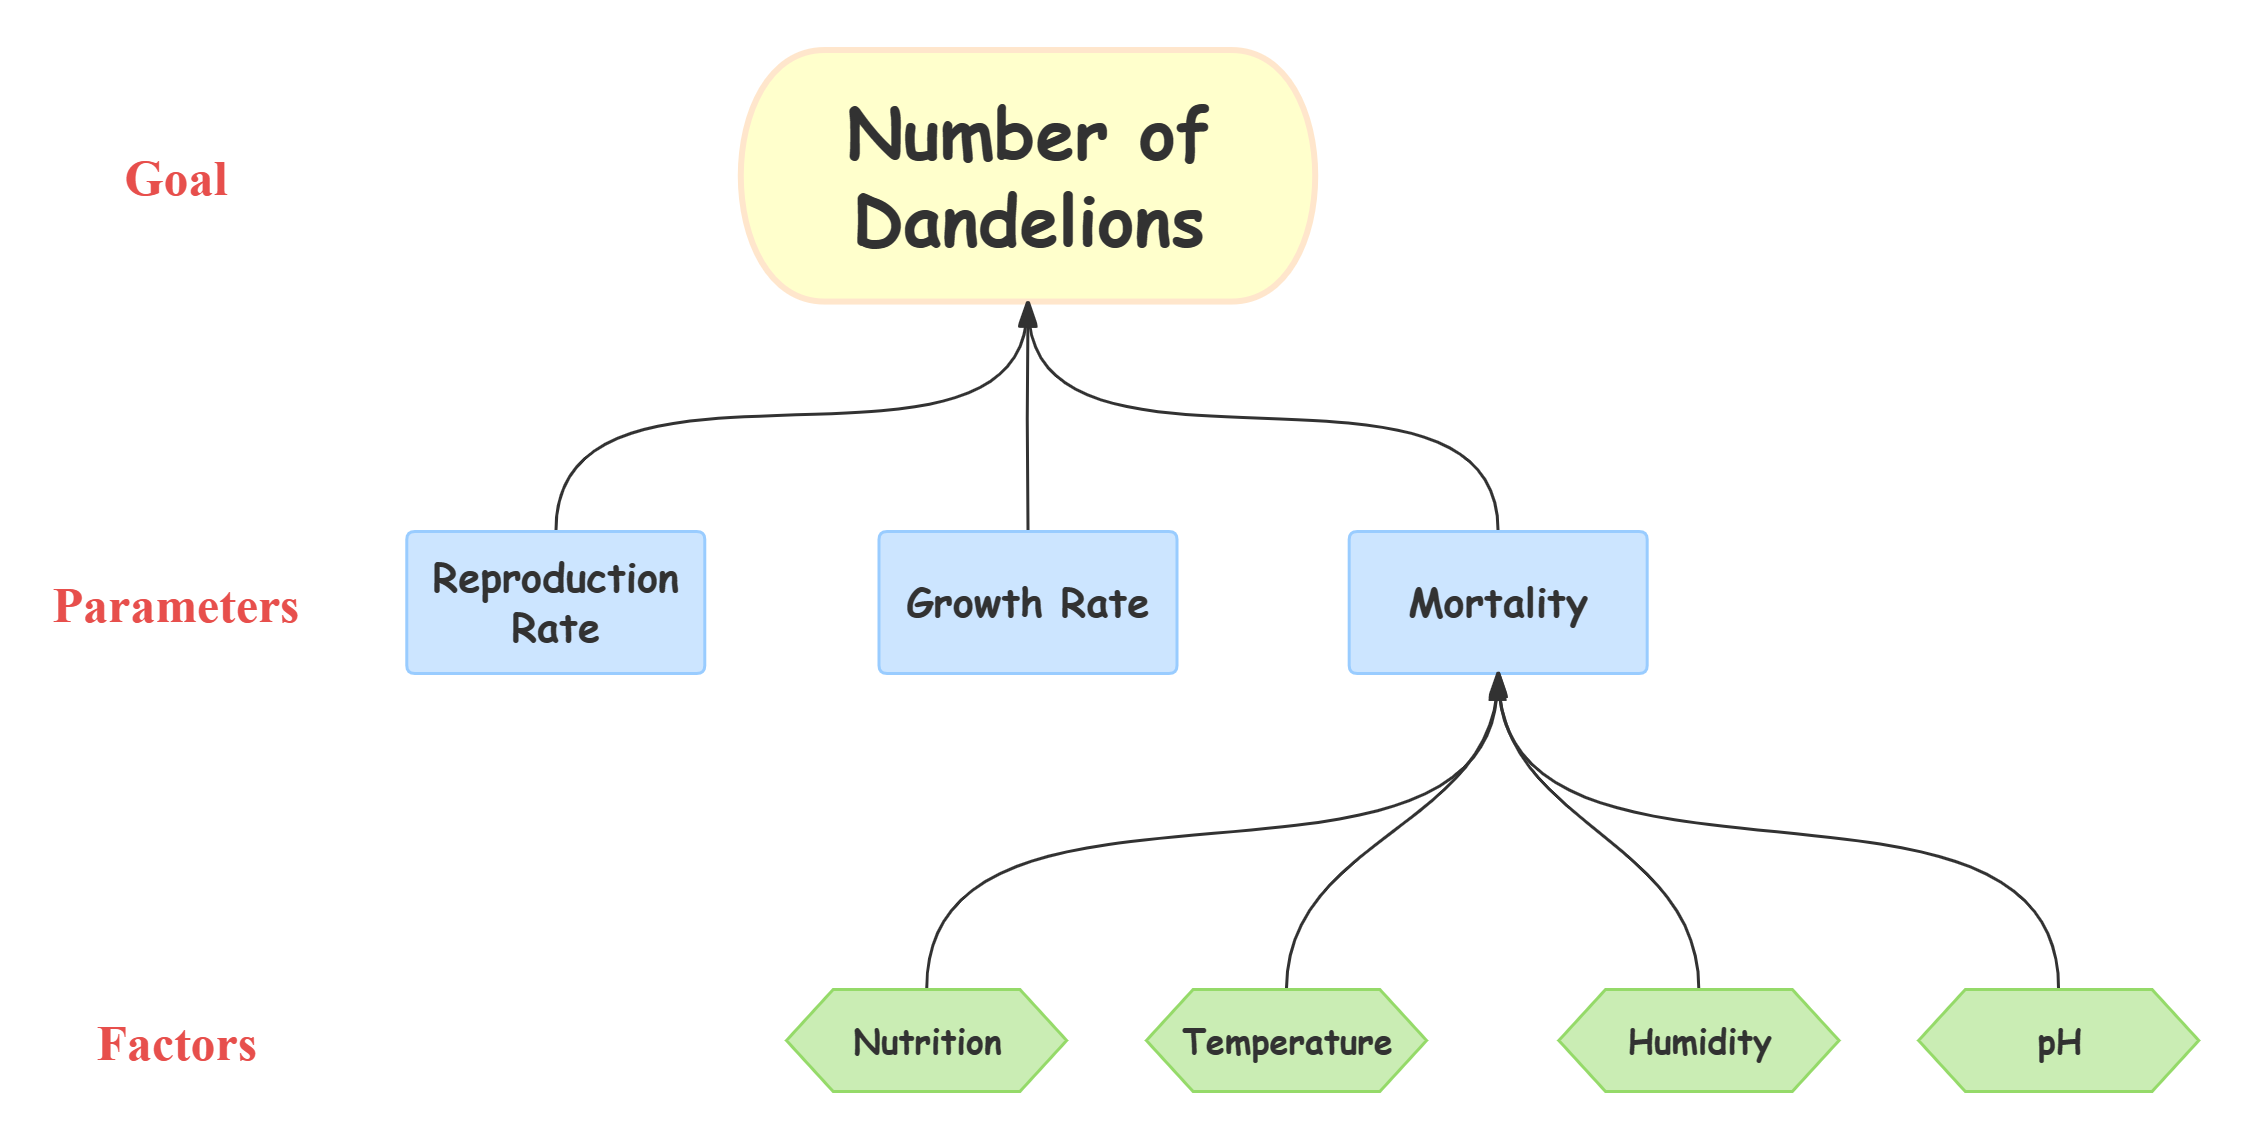
\includegraphics[width=0.6\linewidth]{img/flowchart.png}
    \caption{Structure of Differential Equation Model}
    \label{Structure}
\end{figure}
The overall structure of our differential equation model is shown in \hyperref[Structure]{Figure \ref*{Structure}}. Clearly from the figure, our model is divided into three levels - goal, parameters, and factors. Concretely speaking, our final objective is to find the expression for the number of dandelions. To achieve this, we examine the whole process of the dandelion from growth to death and thus introduce three parameters - reproduction rate, growth rate, and morality. Going further, these parameters are affected by various environmental factors. In the following parts, we will elaborate on the relationship between the three levels in the form of functions and equations.

\subsection{Equations for the Number of Dandelions}
Comprehensively considering all kinds of factors, we have constructed the following equations for the number of dandelions.
\begin{equation}
    \begin{aligned}
    N&=S+P,\\[0.5em]
    \frac{\mathrm{d}S}{\mathrm{d}t}&=\mu_rP-\mu_{m,s}S-\mu_gS,\\[0.5em]
    \frac{\mathrm{d}P}{\mathrm{d}t}&=\mu_gS-\mu_{m,p}P.
    \end{aligned}
\end{equation}
where $N$ denotes the total number of dandelions, $S$ and $P$ denote the number of seeds and puffballs respectively. Here, we divide the total number of dandelions into two stages, the number of seeds and the number of puffball stage dandelions, without losing the generalizability. In the list of differential equations, \(\mu_r P\) represents the number of seeds increases due to the reproduction of dandelions. \(\mu_gS\) represents the process of seeds growing to the puffball stage, which decreases the number of seeds and increases that of puffball. \(\mu_{m,s} S\) and \(\mu_{m,p} P\) represent the death of seeds and puffballs for various reasons, respectively.

\subsection{Parameters and Environmental Factors}
\subsubsection{Expression for Parameters}
In this section, we manage to find the specific expression for each parameter in differential equations, \(\mu_r,\mu_g,\mu_{m,s}\) and \(\mu_{m,p}\).

\paragraph{Reproduction Rate}
We suppose the number of seeds each dandelion can reproduce to be \(n_r\), and the total time of this process to be \(t_r\). Then our reproduction rate can be expressed as \(n_r t_r^{-1}\).

To consider a more practical situation, we introduce another multiplier, the probability of successful reproduction, \(p_s\), meaning we eliminate the situation in which seeds are reproduced by puffballs but do not end up growing properly in soil for for some reason such as being intercepted by the grass or blow off the field by wind. Hence, our reproduction rate is 
\begin{equation}
    \mu_r=\frac{p_s n_r}{t_r}.
\end{equation}
On average, each dandelion reproduce \(1000\) to \(2000\) seeds per year \cite{kershaw_getting_nodate}. And the probability seeds are not intercepted would be in the range of \([0.11, 0.24]\) with median \(0.17\) \cite{doisy_weed_2014}. It implies the range of \(\mu_r\) is \([0.30, 1.32]\).

\paragraph{Growth Rate}
It takes $t_g$ days for seeds to reach their maturity, the puffball stage, so the average growth rate per day per number of dandelions is \(t_g^{-1}\). That means we have
\begin{equation}
    \mu_g=\frac{1}{t_g}.
\end{equation}
Commonly, it takes dandelion seeds about \(60\) to \(95\) days to blossom, and subsequently, \(9\) to \(15\) days to grow into puffballs \cite{eve_how_2023}\cite{maria_its_nodate}. Thus, a reasonable range for $t_g$ is $ \left[75,105\right]$. It implies the range of $\mu_g$ is $\left[0.0095,0.0133\right]$.

\paragraph{Mortality for Seeds}
As a seed grows, it may die for a variety of reasons, including unsuitable temperatures, humidity, pH, and other environmental factors, which act as a multiplying factor \(\alpha\) in the expression of seed mortality. Furthermore, concerning the nutrition factors for seeds are dependent on the resource level, we used the notation $\alpha_{n,p}$ to describe its effect. That means we have
\begin{equation}
    \mu_{m,s}=1-(1-\alpha)(1-\alpha_{n,s}).
\end{equation}

\paragraph{Mortality for Puffballs}
The mortality of puffballs has similar influence factors to that of seeds. However, we distinguish the factor of lack of nutrition for puffballs, \(\alpha_{n,p}\), from that for seeds, and factor in the natural death rate of puffballs, so that the expression is
\begin{equation}
    \mu_{m,p}=1-(1-\alpha)(1-\alpha_{n,p})+\frac{1}{t_d} ,
\end{equation}
where $t_d\in [450,510]$ is the time taken for the dandelion to die from its puffball stage.

In this section, we elaborate on environmental factors that affect mortality, namely \(\alpha\), $a_{n,s}$, and $a_{n,p}$ as above.

\subsubsection{Resource Level}
We define the Resource Unit as the resource accumulated by $1$ Square Meter of land in $1$ normal Day, without losing the generalizability. Thus, in a hectare of land, $R_e=10000$.

We introduce the resource level to measure the amount of nutrition in the land. The following formula gives the differential equation for that:
\begin{equation}
    \frac{\mathrm{d}R}{\mathrm{d}t}=R_e+\kappa \mu_{m,p}PR_d-\lambda_s SR-\lambda_p PR,
\end{equation}
where $\lambda_s$ and $\lambda_p$ are the proportion of resources absorbed by one seed and puffball each day, respectively; $R_d$ denotes the resources accumulated by each dead dandelion in its lifetime; and $\kappa$ donates the total amount of resources given out by the death of the dandelion to the total amount of resources it absorbs throughout its lifetime.

\subsubsection{Nutrition}

\paragraph{For Seeds}
Lack of nutrition is one of the main factors bringing about the death of seeds. It may be affected by the actual resource level of the land as well as the competition among plants. Considering the difference in biomass and nutrition demand between seeds and puffballs, we let the ratio of the resource cost by puffball to the resource cost by seed be 
$\frac{\lambda_p}{\lambda_s}$. Therefore, the equivalent number of seeds which consume the same level of resource can be written as
\begin{equation}
    S_{\text{eq}}=S+\frac{\lambda_p}{\lambda_s}P.
\end{equation}
We incorporate the activation function to describe the relationship dependent on resource level per seed $\frac{R}{S_{\text{eq}}}$ and mortality. Here, we assign the logistic function as 
\begin{equation}
    \alpha_{n,s}=\frac{1}{1+e^{k\left(\frac{R}{S_{\text{eq}}}-\frac{\lambda_s}{\lambda_p}R_{\text{cri},p}\right)}},
\end{equation}
where $k$ is a positive constant, and $\frac{\lambda_s}{\lambda_p}R_{\text{cri},p}$ means the critical resource required for a seed. We can see clearly from \hyperref[Nuitrition]{Figure \ref*{Nuitrition}} that as the resource per seed decreases beneath the critical level, $\alpha_{n,s}$ will rapidly increase to $1$, leading the dandelions to a more vulnerable stage.

\begin{figure}[h]
    \centering
    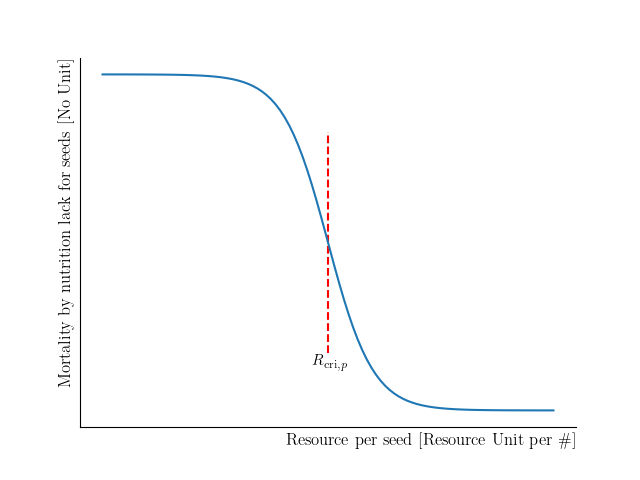
\includegraphics[width=0.5\linewidth]{img/nutrition.png}
    \caption{Logistic Function}
    \label{Nuitrition}
\end{figure}

\paragraph{For Puffballs}
Similarly, the equivalent amount of puffballs, $P_{\text{eq}}$, is expressed as
\begin{equation}
    P_{\text{eq}}=P+\frac{\lambda_s}{\lambda_p}S,
\end{equation}
applying the same activation function, we obtain
\begin{equation}
    \alpha_{n,p}=\frac{1}{1+e^{k\left(\frac{R}{P_{\text{eq}}}-R_{\text{cri},p}\right)}}.
\end{equation}

\subsubsection{Other Environmental Factors}
\begin{wrapfigure}{r}{0.5\textwidth}
	\centering
	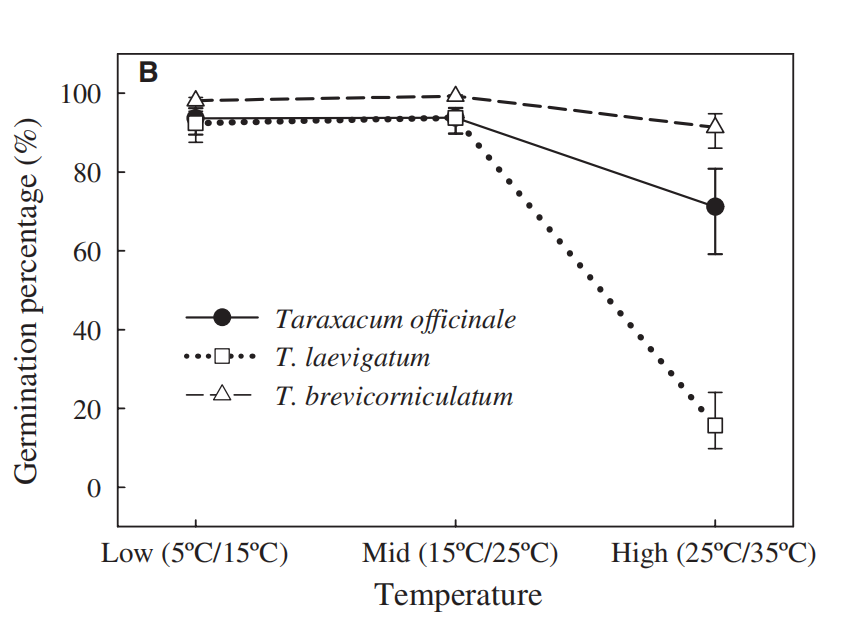
\includegraphics[width=0.7\linewidth]{img/Temp.png}
	\caption{Temperature vs. Survival Rate}
	\label{temp}
\end{wrapfigure}
\paragraph{Temperature}
% \begin{figure}[h]
As \hyperref[temp]{Figure \ref*{temp}} illustrates, we found that dandelions are intolerant to high temperatures \cite{luo_germination_2012}. Thus, we assign $\alpha$ suddenly increases to $1$ in extreme heat, namely above $\SI{25}{\degreeCelsius}$. Beneath $\SI{25}{\degreeCelsius}$ is the safer range, $\alpha$ slowly increases to $1$ at the lefthand side. In the optimal range, $\alpha$ will be a value close to $0$, meaning the temperature is suitable for the dandelion to grow.

\paragraph{Humidity}
Humidity is one of the factors that accounts for the population of dandelions. Dandelions can survive even in harsh environments, where the humidity is relatively low \cite{idris_yau_learn_2022}. That is to say, although decreasing humidity under the range might increase $\alpha$, the extent will not be dramatic. Furthermore, dandelions do not require a high level of humidity to thrive, meaning that $\alpha$ can maintain a low value for a wide range. The dandelion is not sensitive to the humidity, so the impact of the humidity on the dandelion is relatively small.

\paragraph{pH}
We found that dandelions can survive with pH in \([6.0,8.5]\) and the optimal range is \([6.2,6.8]\) \cite{dekker_how_2021}. Thus, we assign $\alpha$ closer to $0$ in the optimal range, since the dandelion will have a smaller chance to die if the pH value is in their comfortable range. On the other hand, if the pH value is extreme, either too acidic or too basic, the mortality of dandelion $\alpha$ rapidly increases to $1$.

\subsection{Results and Variations of the Differential Equation Model}
\begin{wrapfigure}{r}{0.5\textwidth}
    \centering
    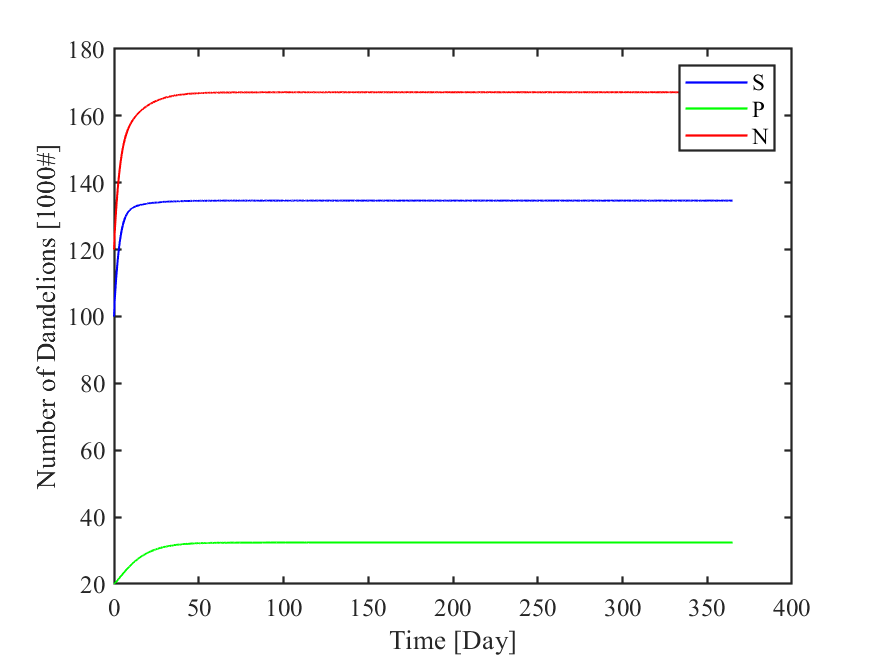
\includegraphics[width=0.5\linewidth]{img/100-20.png}
    \caption{Result of Basic Case}
    \label{basic}
\end{wrapfigure}
In this section, we are going to display the result, in the form of images of functions, solved by the differential equation model, as well as analyze the result.


\subsubsection{Basic Case}
For the most basic case, we let \(S=100, P=20\) at the beginning, and the result is shown in \hyperref[basic]{Figure \ref*{basic}}. We can observe that the number of seeds slightly increased at first but soon came back to \(100\), while that of puffball steadily rose to \(60\) before reaching an equilibrium state.


\subsubsection{Different initial condition}
We have changed the initial number of dandelions in both stages and obtained the result in \hyperref[diff_ini]{Figure \ref*{diff_ini}}, which considers the special cases in which there is no seed or no puffball initially. We found that similar to the base case, the most significant change occurs in the first 50 days, approximately. On top of that, the situation in which no initial seeds, For example, in the second graph, ends up the same value as the basic case. In contrast, if there are no puffballs at first, there will be eventually more dandelions but fewer puffballs.
\begin{figure}[h]
  \centering\begin{subfigure}[b]{0.45\textwidth}
    \centering
    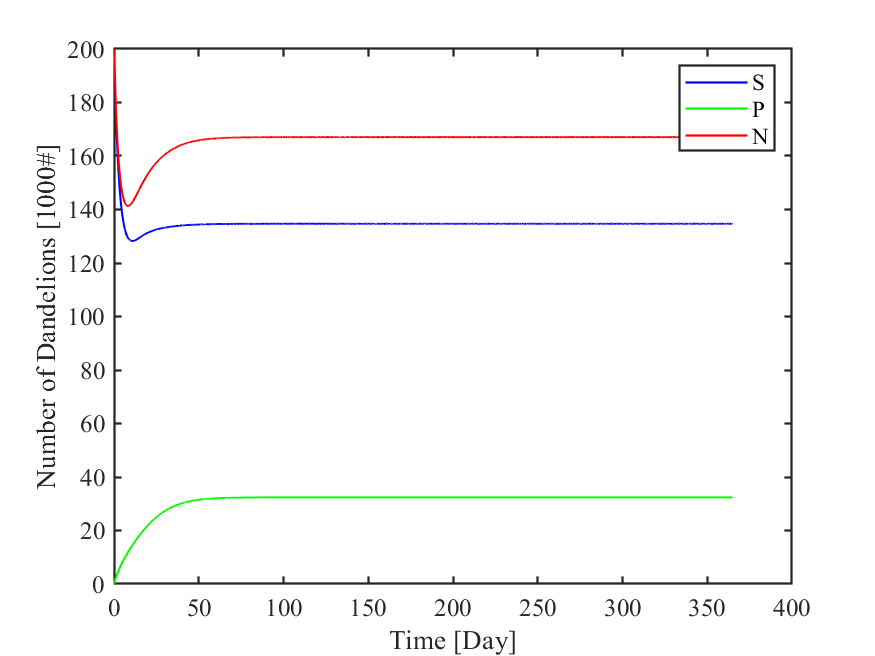
\includegraphics[width=0.7\textwidth]{img/200-0.png}
  \end{subfigure}
  \quad
  \begin{subfigure}[b]{0.45\textwidth}
    \centering
    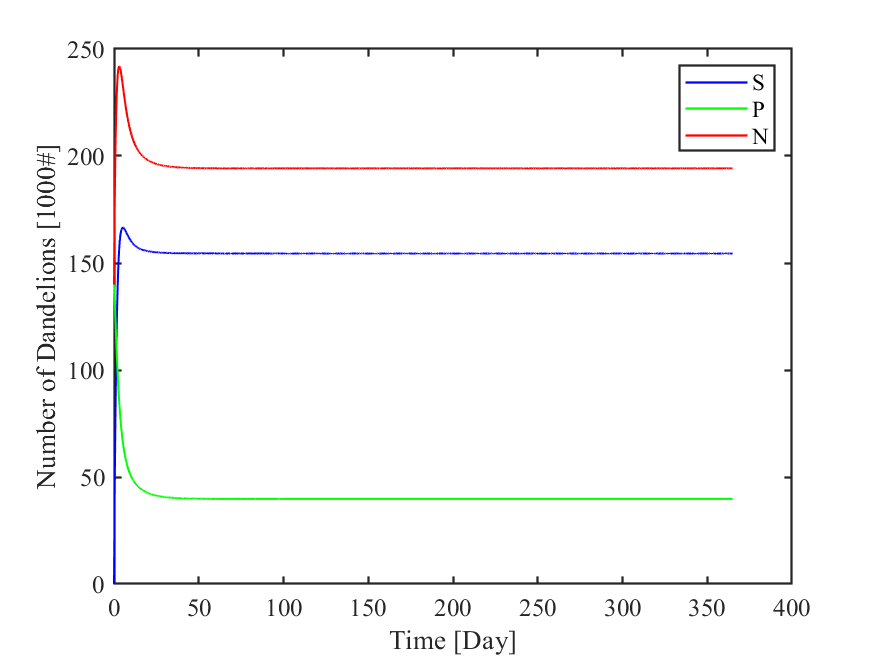
\includegraphics[width=0.7\textwidth]{img/0-140.png}
  \end{subfigure}
  \caption{Results under Different Initial Conditions}
  \label{diff_ini}
\end{figure}

\subsubsection{Different environmental factor}
Additionally, we also want to study the situation under different environmental factors, taking into account the change in temperature and humidity, among others.

\paragraph{Dry Conditions} Firstly, we simulate the dry conditions. Thereinto, we decrease the value of \(\lambda_s\) and increase \(\alpha\) slightly, for the sake of increasing the mortality of dandelions, particularly seeds, under such conditions, according to \cite{wigg_dandelion_nodate}. Moreover, we also reduced the value of \(\kappa\) since a dry environment would inhibit the biodegradation, thus resulting in less nutrient transfer to the soil from dead dandelions \cite{joly_resolving_2023}. We can see in the first graph of \hyperref[diff_env]{Figure \ref*{diff_env}} that, the total number of dandelions is, as expected, lower than that in \hyperref[basic]{Figure \ref*{basic}}, with both numbers of seeds and puffballs experiencing a decline. However, we also notice that the difference is not significant.

\paragraph{Tropical rainforest climate} Then we analyze a more complicated situation - the tropical rainforest climate, characterized by high temperature and humidity and numerous plants. Hence, we assign \(\alpha\) to a relatively high value since excessive temperature and humidity are not good for the growth of dandelions. Additionally, dandelions are not able to obtain enough sunlight due to the shade of numerous tall plants, which may affect their growth \cite{dekker_how_2021}. Despite that, to conform with reality, we increase the initial resources and resources added by the environment. Clearly from the second graph in \hyperref[diff_env]{Figure \ref*{diff_env}}, the total number of dandelions is significantly lower than that under other conditions, meaning that it is a relatively unsuitable position for the growth of dandelions.
\begin{figure}[h]
  \centering\begin{subfigure}[b]{0.45\textwidth}
    \centering
    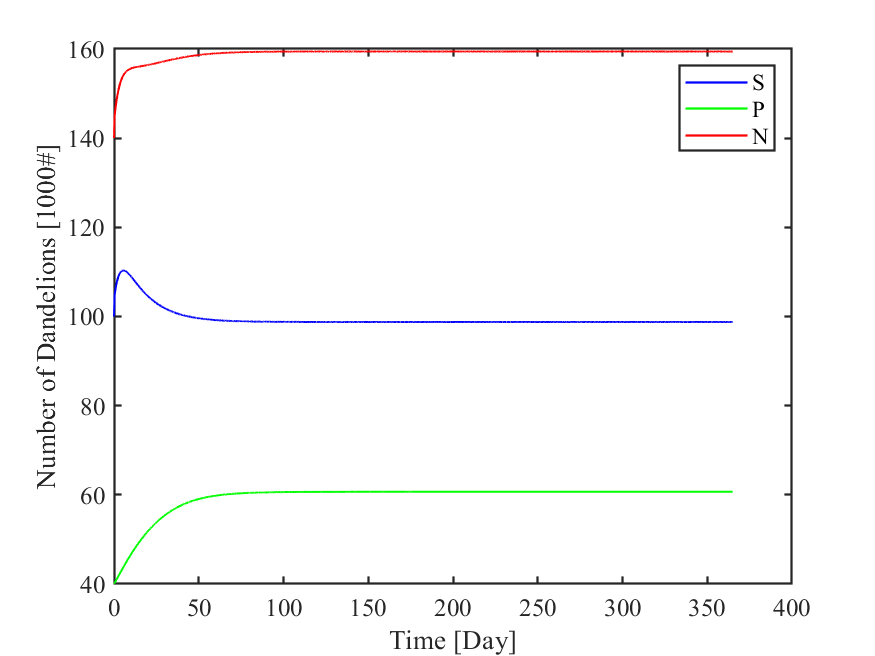
\includegraphics[width=0.7\textwidth]{img/dry.png}
  \end{subfigure}
  \quad
  \begin{subfigure}[b]{0.45\textwidth}
    \centering
    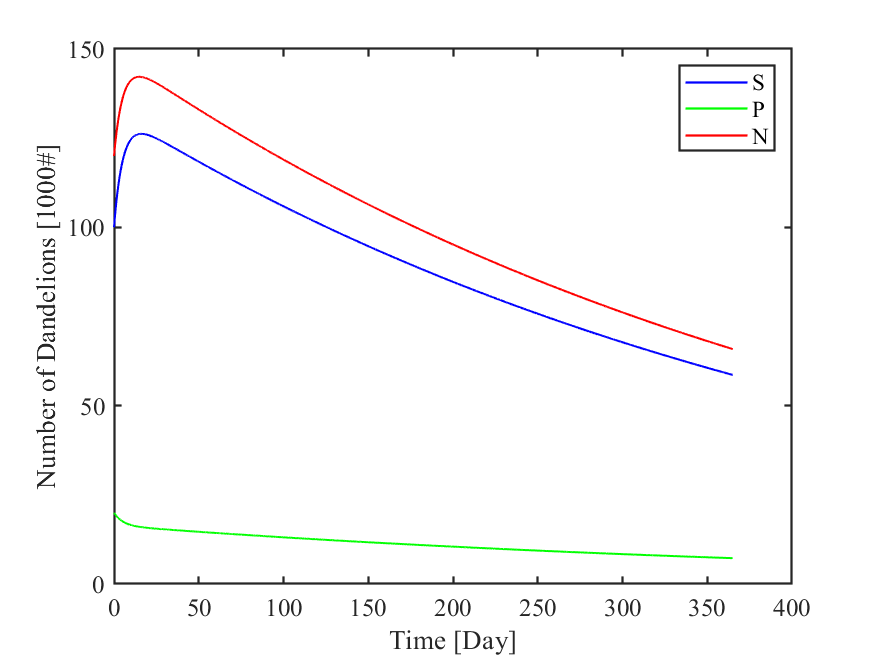
\includegraphics[width=0.8\textwidth]{img/tropical.png}
  \end{subfigure}
  \caption{Results under Different Environmental Factors}
  \label{diff_env}
\end{figure}

\section{Cellular Automaton Model}
Cellular Automaton (abbr. CA in the following), can also be used in the modeling of dandelion dynamics. Unlike the differential equation model, the CA model focused on the individuals rather than the dandelion population as a whole. Thus, beyond the differential equation model, we can manipulate regional factors such as seed distribution, puffball distribution, the shape of the field, and small differences in resources across the field. Via these complements, CA is capable of the prediction of more complex patterns and situations, such as periodic behaviors, or inter-plant influences.

In contrast with the differential equation model, the cost of the precise predictions on individuals is discontinuity. In the classical CA, time $t$ and space $ l$ are discontinuous and in lattices. The approach we made is to increase the ``resolution" of the lattices to desalinate the effects of the discontinuity.

\subsection{The Basises of the Cellular Automaton Cells}
Dividing our dandelion field into square lattices of length of $ l$, each CA cell symbolizes a piece of field. Thus, each grid contains two pieces of major information: the state of the plant, if it has one, and the resources level. In our model, we use the side length of $ l=0.01$ for the following stimulation.

\subsubsection{Parameters for Dandelion}
In the simulation, let $t_i$ represent the time that has elapsed since the seeding of dandelion $i$. It takes $t_g$ days for a seed to grow up into a puffball. After that, the puffball has a reproduction window that lasts for $t_r$ days. The seeds are dispersed to the neighbor cells, not necessarily adjacent, triggering the next life cycle. Afterward, the dandelion maintains its puffball stage for \(t_d\) days before its death. We thus divided the life span of a dandelion into two phases: $t_i\in \left[0,t_g\right]$ for the first phase and $t_i\in \left[t_g,t_g+t_d\right]$ for the second phase.

The radius of the dandelion root at time $t_i$ after its seeding is captured by $r_{t_i}$, where $r_0=0$ since a seed has not yet developed its rooting system. For the first phase, we assume its root is developed linearly to time, meaning
\begin{equation}
    r_{t_i}=\frac{t_i}{t_g}r_p
\end{equation}
and stay at $r_p\in [0.152, 0.305]$ meters for phase two \cite{mahr_dandelion_nodate}.

\subsubsection{Resources Level}
The resource level represents the concentration of nutrition in each cell, noted $R_{(x,y)}$ for the cell located at $(x,y)$. Due to the external resources' replenishment, the resource level automatically increases. A dandelion plant has access to the resource in cells whose distance to the plant is less than or equal to the root radius $r_{t_i}$. Due to the dandelions' absorption, the resource level nearby decreases. We assume the absorption rate is proportional to the level of resources $R_{(x,y)}$ - the less nutrition a grid has, the less it absorbs. The total resources absorbed in day $t_i$ for a specific dandelion is noted $R_{t_i}$.

Lack of resources will lead to the death of the plant, so we assign the plant a critical resource level $R_{\text{cri},t_i}$ as the minimum resource they need to obtain at day $t_i$. We assume the bond is quadratic to time in phase one:
\begin{equation}
    R_{\text{cri},t_i}= \frac {t_i^2}{t_g^2}R_{\text{cri},p},
\end{equation}
where $R_{\text{cri},p}$ is a constant representing the amount of resources necessary for a puffball-stage dandelion. Then, $R_{\text{cri},t_i}$ will remain at $R_{\text{cri},p}$ for the second phase.

If $R_{t_i}$ is lower than $R_{\text{cri},t_i}$, then the dandelion is facing the risk of death. We sketch a logistic function centered at $R_{\text{cri},t_i}$ to symbolize the death rate due to lack of natural resources $\alpha_{n,s}$ and $\alpha_{n,p}$ for these malnutritional dandelions. Thus,
\begin{equation}
    \alpha_{n,s}=\alpha_{n,p}=\frac{1}{1+e^{k\left(R_{t_i}-R_{\text{cri},t_i}\right)}},
\end{equation}
where \(k\) is a constant, defined similarly in the differential equation section. As for the calculation of $\mu_{m,s}$ and $\mu_{m,p}$, it is the same expression as the previous model as well, hence we will not go into detail here.

Whenever a dandelion dies, no matter in which phase, it fertilizes its surroundings. The total amount of resources given out by the death of the dandelion is proportional to the total amount of resources it absorbs throughout its lifetime. We denoted this coefficient $\kappa$.

\subsubsection{Additional Factors}
Here we will discuss some additional factors beyond the differential equation model.

\paragraph{The Shape of the Field}
We considered two types of fields in two extremes, one with long boundaries and one with short boundaries to keep the comparison simple. Since the boundaries will cause the loss of seeds in reproduction, land with longer boundaries will have a lower successful seeding rate, ignoring the effect of wind bias on the distribution of seeds. To keep it simple, we will run two simulations, one with periodic boundaries and the other with open boundaries, imitating the land with short boundaries and long boundaries, correspondingly.

For short-boundary land, periodic boundaries compensate for insufficient computing power by ignoring the edge effect, without losing the generalizability. It means that the seeds flying across the northbound will be at the southbound, and the same algorithm connected the eastbound and the westbound.

The open boundaries, on the other hand, make consideration on the edge of the land, since the seeds flying across the edge will lost forever. Since dandelions cannot be planted outside of the land, the number of seeds by reproduction and resources distributed are not as same as the interior, this boundary condition suits the long-boundary lands better.

\paragraph{Initial Seed \& Puffball Distribution}
In this section, we will analyze how the distribution of dandelion affects the results. Here, we compare two typical distributions: uniform distribution, and the distribution simulating the dandelion invasion.

Uniform distribution is the simplest distribution, the dandelion is distributed evenly across the field with the natural density $\rho_0=14.8\pm 4.9$ \cite{eggert_yield_2018}. The behavior of dandelion should be similar across the field. Due to the solvability limit, we focus on a square section of the field, with the side length of $2^{12} l$.

To find out the invasions that take place in the dandelion, we just need to focus on the frontline of the dandelion invasion. Thus, in the ``invasion"-type distribution simulation, we give the right half of the field an even distribution of density $\rho_0$, whereas the left half of the field is a wasteland, with no dandelion on it. The northbound and the southbound are still connected as periodic boundaries, due to the consistency of the vertical direction, but the eastbound and the westbound, on the coin side, are open boundaries.

\paragraph{Resources Distribution}
In reality, resources are not evenly distributed and some regions will be richer than others. Thus, we have considered three distributions of resources, which are the uniform distribution, the trendliness distribution, and the random distribution to approach the distributions of resources in real-life circumstances. The illustration of these distributions is shown in \hyperref[Distributions]{Figure \ref*{Distributions}}.
\begin{figure}[h]
    \centering
    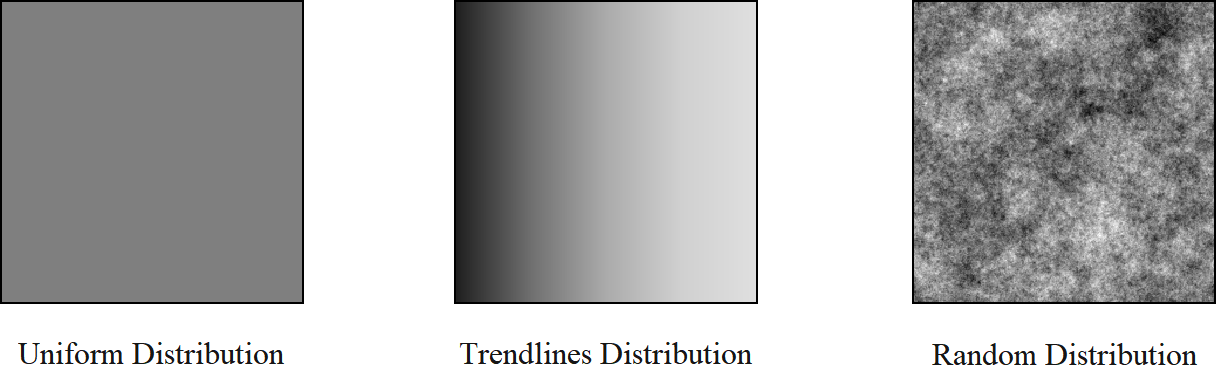
\includegraphics[width=0.5\linewidth]{img/Distributions.png}
    \caption{Vivid Illustrations of the Distributions}
    \label{Distributions}
\end{figure}

Uniform distribution is the trivial case, in which the resource is distributed identically on each cell. Thus, in mathematical convention, for all $(x,y)$, $R_{(x,y)}=R_0$, the resource in each cell, at $t=0$.

Trendline distribution is simply linearly assigned the resource level to each cell. The resource is rich on one side, and poor on another. By this approach, we can observe the dependency of dandelions on the resource level.

Random distribution is a more realistic approach because we introduce $2$-dimensional pink noise adding the original level, creating some local fluctuation. Since pink noise gives some level of dependence on the resource level in adjacent CA cells, it is more realistic than randomly assigning values in a range to the CA cells independently.

\subsection{Cellular Automaton Modeling, Rusult, and Analysis}
\begin{figure}[h]
    \centering
    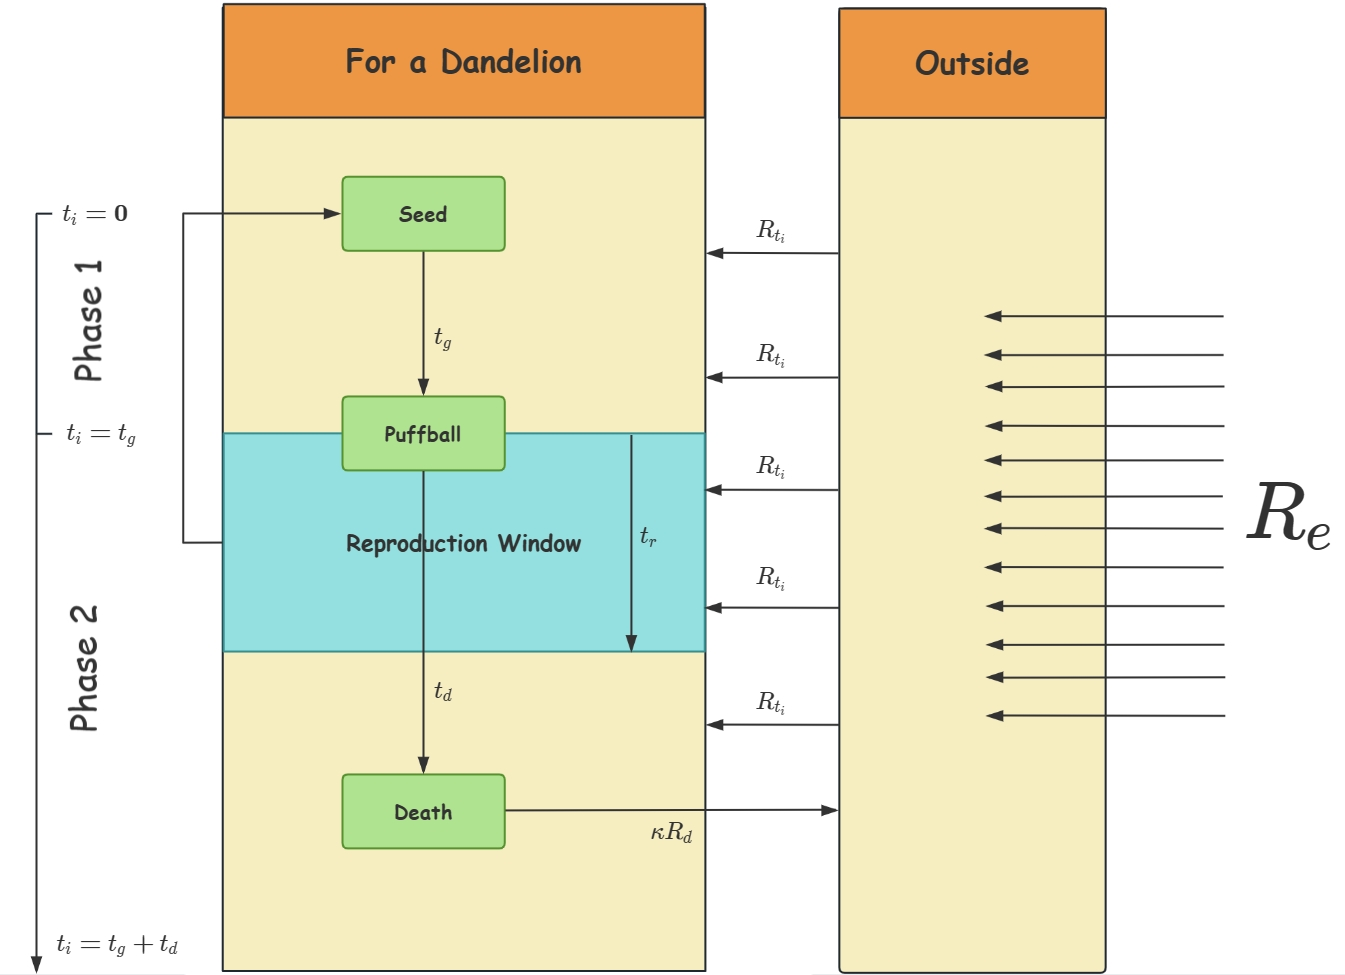
\includegraphics[width=\linewidth]{img/process.png}
    \caption{Flow Chart of the Working Process of CA Model}
    \label{process}
\end{figure}

\subsubsection{Comparison among Various Parameters}

\paragraph{Different Initial Seed \& Puffball Distributions}
The two possible distributions are uniform distribution and ``invasion"-type distribution. Uniform distribution strictly follows the natural density $\rho_0$, while in the ``invasion"-type distribution's situation, we assume that half of the open area has reached $\rho_0$ and life cycles will take place here. However, the rest half the area, will remain open. Contrasting the two propagation modes, uniform distribution means dandelions would start the life cycle on the area evenly, while ``invasion"-type distribution means dandelions would first invade certain areas, then another area. 

\paragraph{Different Resources Distributions}
The three possible distributions are uniform distributions, trendlines distributions, and random distributions. In real-life situations, the distribution of nutrients would incorporate all of them. As dandelions' growth absorb nutrients, dead dandelions add nutrient, and the natural nutrient accumulating process, the resource distribution becomes less even. The different distribution of resource levels will lead to the nonuniformity of dandelions. 

\subsubsection{Periodic Behaviors}
A dandelion adjacent to the land, which is ready for propagation is the start of the life cycle. Seeds have spread either uniformly or through invasion, and they start growing, absorbing $\lambda_{t_i}$ resources from the soil every day. At the same time, nutrient $R_e$ is added to the environment per day. Soon the dandelions mature and step into the puffball stage, in which $\lambda_{t_i}$ resources are absorbed. After the seeds are carried by wind to nearby areas, the old dandelions die and give back $R_d$ nutrients to the soil. The life cycle repeats on the land, resulting in the continuing propagation of dandelions. 

\subsubsection{Inter-Plants Influences}
Plants compete with each other for resources. When the resources absorbed by dandelions is much larger than the resources added to the environment, the soil loses nutrient, and some plants may not absorb enough $R_{cri,p}$. In consequence, they will not enter the puffball stage. 

\section{Evaluation of Invasive Species}
Despite the advantages dandelions can bring us, many classify dandelions as an invasive species. In this section, we developed a model, combining the Analytic Hierarchy Process (abbr. AHP in the following), and differential equation, and concentrated on the vulnerability of the original species to analyze and determine whether dandelions are considered invasive species. We will consider the interaction of two species to stay simple and practical, without loss of generality.

\subsection{Interspecies and Intraspecies Competition for Resources}
The following differential equations can characterize the extent of invasiveness:
\begin{equation}
\begin{aligned}
N & = A+B \\[0.5em]
\frac{\mathrm{d}A}{\mathrm{d}t} & = \frac{A\left(\gamma_1-\gamma_3 B\right)\left(A_{\max} -A\right)}{\gamma_5 \left(N+\gamma_6\right)}\\[0.5em]
\frac{\mathrm{d}B}{\mathrm{d}t} & = \frac{B\left(\gamma_2-\gamma_4 A\right)\left(B_{\max} -B\right)}{\gamma_5 \left(N+\gamma_6\right)}
\end{aligned}
\end{equation}
where $A$ and $B$ denote the population of native and invasive plants. $N$ is the total population of native and invasive plants. $\gamma_1$ and $\gamma_2$ are the growth rates of each species. $\gamma_3$ and $\gamma_4$ denote, respectively, the inhibition by one invasive plant to all native plants and the inhibition by one native plant to all invasive plants, due to interspecies competition. Considering intraspecies competitions, we use $A_{\max}$ and $B_{\max}$ to represent the maximum capacity one species can be held in the system. $\gamma_5$ is a time coefficient, which is affected by the rate the system interacts. $N+\gamma_6$ on the denominator symbolizes resource competition, where $\gamma_6$ is the number of individuals other than native and invasive, but still consuming the resource. When $N$ is large enough, it would likely cause competition for resources.

Then let us consider how these coefficients would affect the results. We divided the possible outcome into four cases:

\paragraph{Case 1: Convergence to Stable Points} When $A=\frac{\gamma_2}{\gamma_4}$, $B=\frac{\gamma_1}{\gamma_3}$, $\frac{\mathrm{d}A}{\text{d}t}=\frac{\mathrm{d}B}{\text{d}t}=0$, the system goes to a balanced status. When $A$ and $B$ are not in the stable level, which is the common case, the differential equation will still have a chance to reach the stable level. If the initial condition is in its convergence basin, then it will still converge, approaching the stable point $(\frac {\gamma_2}{\gamma_4},\frac {\gamma_1}{\gamma_3})$ in the system. In this paper, we will not consider a point stable if one of the species is $0$, and this situation is described below.

\paragraph{Case 2: One Species Driven out The Other} In some of the initial conditions, when one species has a significant advantage over the other, it may drive the other out of the system. This is saying, that in case the foreign species repels the native one, the native species approaches $0$. Namely, if this is the case, $A$ approaches $0$ as $t$ approaches $\infty$, namely
\begin{equation}
    \lim_{t\to \infty} A=0.
\end{equation}
On the other way around, we also put the result where the natives finally executed the foreigners into this case.
       
\paragraph{Case 3: Oscillations} 
In this case, in general, the system is in a dynamic state, neverendingly but regularly. That means, A and B alternatively surpass the other one, which forms a dynamic equilibrium. Academically speaking, as $t\to\infty$, the system tends to become periodic and the same scenario would appear over and over again. Commonly, the situation classified in this case is that one factor is positively correlated to the other, but the other factor is negatively correlated to the first one.

\paragraph{Case 4: Chaos} This case indicates the dynamic will never converge to a stable, predictable pattern. We classify all the unpredictable patterns here, so we will not discuss this case in depth in this paper.

The parameter space of $A$ and $B$ and its trajectory lines due to time are shown in \hyperref[Trajectory Lines]{Figure \ref*{Trajectory Lines}}.
\begin{figure}[h]
    \centering
    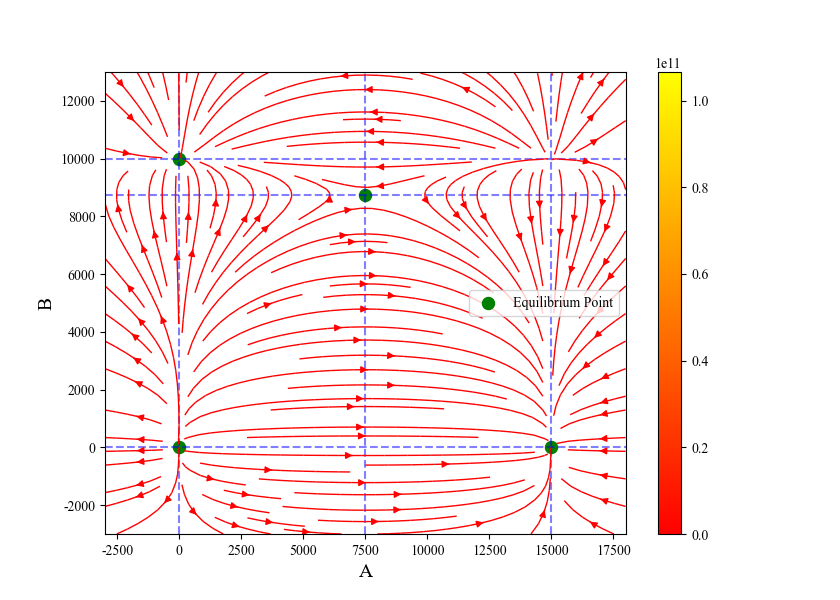
\includegraphics[width=0.6\linewidth]{img/Trajectory.png}
    \caption{The Trajectory Lines of the Competition between native and invasive plants}
    \label{Trajectory Lines}
\end{figure}
We can examine the value of $\frac{\gamma_1}{\gamma_3}$ and $\frac{\gamma_2}{\gamma_4}$, in terms of figuring out the extent of invasiveness. Based on this thought, we will consider how this value would be determined. Besides, through \hyperref[Trajectory Lines]{Figure \ref*{Trajectory Lines}}, we found that the only two stabilize points in the parameter space lay on the axis, meaning that whatever starting condition it is, one of the species will eventually remove the other from the system.

\subsection{Determine the Parameters}
\subsubsection{Plant's Natural Characteristics}
\paragraph{The number of dandelions introduced}
When the initial value of dandelions is beyond $\frac{\gamma_2}{\gamma_4}$, then it becomes \textbf{Case 1}. At the same time, if the initial value is below $\frac{\gamma_2}{\gamma_4}$, then the introduction of dandelions will not cause much threat to the original species.

\paragraph{Dispersal Distance}
The increasing value of the dispersal distance of dandelion is likely to increase the competitiveness of the resource, thus putting more stress on the resource searching for the original species. Moreover, it will take up the place and replace the original species quickly. That is to say, it will result in a high $\gamma_4$ and $\gamma_1$, and a low $\gamma_5$.

\paragraph{Seed Number per Flower}
The seed number is related to resource competition. When the seeds dandelions can produce are enormous, then they will have an advantage in competing for resources, thus having almost the same effect with dispersal distance.

\subsubsection{Environmental Contributors}
\paragraph{Extreme Weather}
Facing extreme weather conditions, dandelions are excellent at enduring them while the original species might face the risks of being undermined by the weather. Hence, $\gamma_2$ decreases dramatically while $\gamma_1$ changes so little that we can assume $\gamma_1$ is unchanged.

\paragraph{Resource Level}
When the total level of resources increases, it is evident that the population of both species will increase proportionally. So in this case, $\gamma_1$, $\gamma_2$, $\gamma_3$, $\gamma_4$ will all increase proportionally.

\subsubsection{Economic Contribution}
\paragraph{Medical Usage}
Dandelions are known as good raw materials for medicinal materials. Taking this factor into consideration, we can compare the value dandelions can bring us when they take up the space where another species could live. Hence we can quantify the extent of harm dandelions would bring us to the economy based on their medical usage.% Need a conclusion

\subsection{Invasion Index Determination}
After classifying the effects of the introduction of dandelions, we can now develop an AHP model to determine the level of invasiveness, as shown in \hyperref[AHP]{Figure \ref*{AHP}}. Instead of directly evaluating the previous effect, we investigate how the three components $\frac{\gamma_1}{\gamma_3}$, $\frac{\gamma_2}{\gamma_4}$, $\gamma_5$ affect the invasiveness and their importance. Then we use the effects in the section above to determine the weight of each component.
\begin{figure}[h]
    \centering
    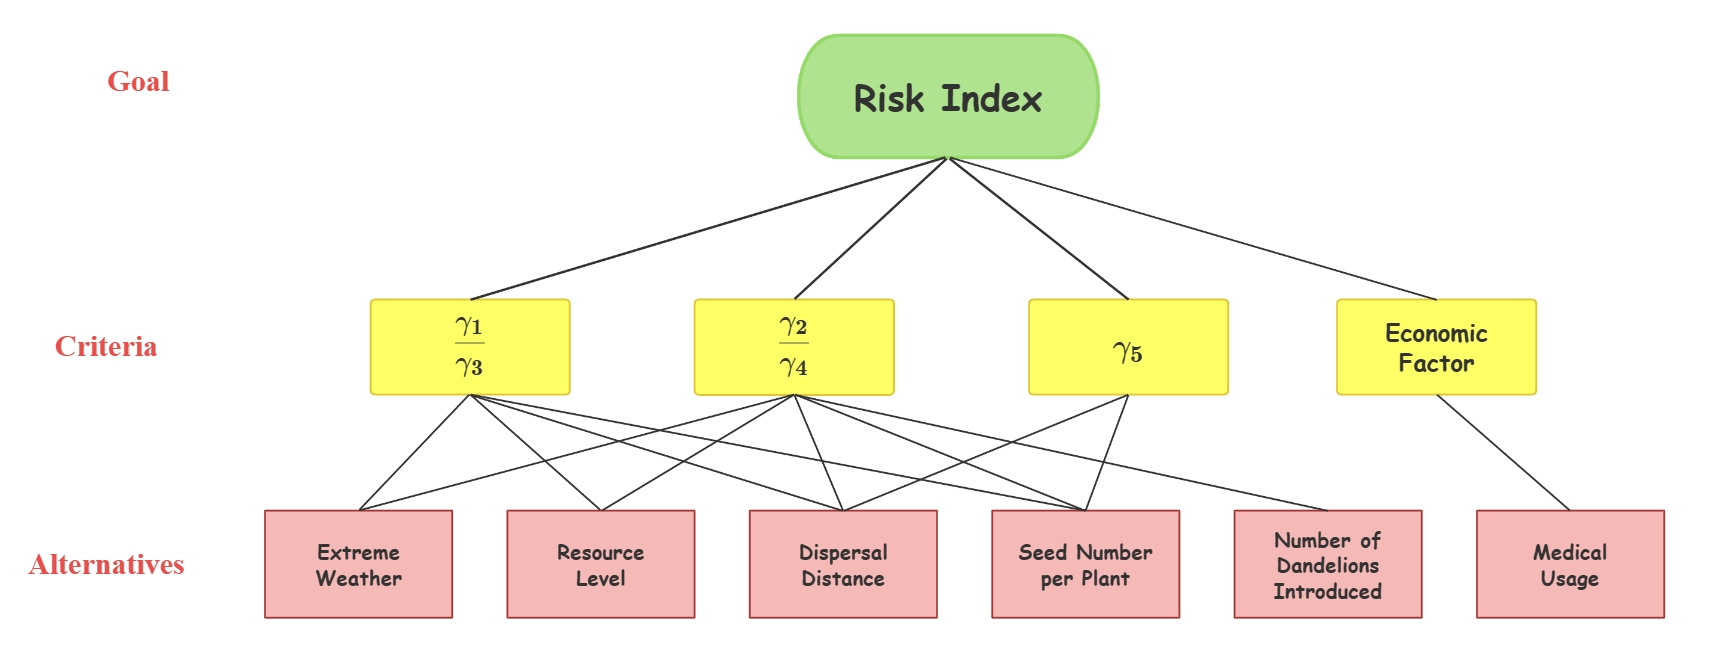
\includegraphics[width=\linewidth]{img/AHP.png}
    \caption{AHP Model}
    \label{AHP}
\end{figure}

\subsubsection{Weights of Three Parameters}
As $\frac{\gamma_1}{\gamma_3}$ and $\frac{\gamma_2}{\gamma_4}$ are symmetric, they are supposed to have equal importance, whereas for $\gamma_5$, we give it a weight $0.8$ compared to other two as the predetermined advantages in competing with each other should outcompete the external exertion of the environment. For the parameters, we consider dispersal distance and seeds per plant as important because they determine the speed of its spread. Then it comes to medical usage because it is quite beneficial to the economy, the next one comes to the resource level as it determines the speed of the spread of dandelions, however, it is restricted to the surrounding condition. The last two are extreme weather and the number of seeds introduced because the number of seeds introduced would not be too much if we control them, and extreme weather does not often occur.
\begin{table}[h]
\renewcommand{\arraystretch}{1.5}
\centering
\caption{AHP Weighting Matrix}
\begin{tabular}{|c|c|c|c|c|}
\hline
Parameters & $\frac{\gamma_1}{\gamma_3}$ &  $\frac{\gamma_2}{\gamma_4}$&  $\gamma_5$&  Weight\\ \hline
$\frac{\gamma_1}{\gamma_3}$ &1&1  &  1.25&  0.35\\ \hline
$\frac{\gamma_2}{\gamma_4}$&1    &    1&  1.25&  0.35\\ \hline
$\gamma_5$&0.8&0.8&1&0.30\\ \hline

\end{tabular}
\label{AHP WM}
\end{table}

\begin{table}[h]
\renewcommand{\arraystretch}{1.5}
\centering
\caption{Judgement Matrix}
\resizebox{0.75\columnwidth}{!}{
\begin{tabular}{|l|c|c|c|c|c|c|c|}
\hline
Parameters & \makecell[{cc}]{Extreme\\Weather}  &  \makecell[{cc}]{Resource\\Level}  &\makecell[{cc}]{Dispersal\\Distance} &\makecell[{cc}]{Seeds\\per plant}&\makecell[{ccc}]{Number of\\Dandelions\\Introducecd}&\makecell[{cc}]{Medical\\Usage}&Weight\\ \hline
Extreme Weather &$1$ &$0.5$ & $0.25$ & $0.25$ &$1$ & $0.3333$ & $ 0.0700$\\ \hline
Resource Level &$2$ &$1$  &  $0.5$ &  $0.5$&$2$ &$0.6667$ &$0.1401$\\ \hline
Dispersal Distance &$4$ & $2$ & $1$ &  $1$&$4$ & $1.3333$ & $0.2548$ \\ \hline
Seeds per plant  &$4$  & $2$ & $1$ &  $1$&$4$ & $1.3333$ & $0.2548$ \\ \hline
Number of Dandelions Introducecd&$1$ &  $0.5$&  $0.25$& $0.25$&$1$ & $0.3333$ & $0.0700$\\ \hline
Medical Usage  &$3$ &  $1.5$&  $0.75$&  $0.75$&$3$ & $1$ & $0.2101$\\ \hline
\end{tabular}
}
\end{table}
Then we can let
\begin{equation}
\begin{aligned}
\mathrm {\mathbf{W_1}} & =
\begin{bmatrix}
0.35&0.35&0.30

\end{bmatrix},\\[0.5em]
    \mathrm {\mathbf{W_2}} & =
    \begin{bmatrix}
 0.0700
    &0.1401
    &0.2548
    &0.2548    
    &0.0700
    &0.2101

\end{bmatrix},
\end{aligned}
\end{equation}
which represents the weight matrix concerning the two groups of parameters. Also, we can assign the dandelion a matrix, representing its character. The matrix is given by the following, with each value belonging to $[0,1]$, showing the extent of its severity. However, the value of medical usage should be one minus this value because it is a positive sign. In this case, we assume that enough dandelions are being introduced and the resource level is relatively moderate. Therefore, we have
\begin{equation}
    \mathrm {\mathbf{v_d}}=\begin{bmatrix}
0.9 &0.5 &0.8
 &0.8 &0.8 &0.1
 \end{bmatrix}.
\end{equation}
For each factor in \hyperref[AHP WM]{Table \ref*{AHP WM}}, it has its own corresponding 0-1 matrix to represent whether it will be affected by external conditions. It should be
\begin{equation}
\begin{aligned}
    \mathrm {\mathbf{M_{\frac{\gamma_2}{\gamma_4}}}} & =\begin{bmatrix}
1 &1 &1
 &1 &0 &0
 \end{bmatrix},\\[0.5em]
 \mathrm {\mathbf{M_{\frac{\gamma_1}{\gamma_3}}}} & =\begin{bmatrix}
1&1 &1
 &1 &1 &0
 \end{bmatrix},\\[0.5em]
 \mathrm {\mathbf{M_{\gamma_5}}} & =\begin{bmatrix}
0 &0 &1
 &1 &0 &0
 \end{bmatrix}.
 \end{aligned}
\end{equation}
The operation for $\iota_d$ is 
\begin{equation}
    \iota_d=\begin{bmatrix}
\mathbf{M_{\frac{\gamma_1}{\gamma_3}}}(\mathbf{v_d^T}\circ \mathbf{W_2^T})
    &\mathbf{M_{\frac{\gamma_2}{\gamma_4}}}(\mathbf{v_d^T}\circ \mathbf{W_2^T})
    &\mathbf{M_{\gamma_5}}(\mathbf{v_d^T}\circ \mathbf{W_2^T})

\end{bmatrix}
\mathbf{W_1^T}+0.2101\cdot 0.1,
\end{equation}
where $\circ$ denotes the Hadamard product. In addition, the weight of medical usage should be added at last because it is a factor not included in the three parameters. Finally, we will get the value as a risk index. For dandelions, the final value we get is
\begin{equation}
    \iota_d=0.5407\cdot 0.35+0.5967\cdot 0.35+0.4077\cdot 0.3+0.2101\cdot0.1=0.5225.
\end{equation}
If we define a value higher than $0.5000$ to be an invasive species, then dandelions should be included in this group.

\subsubsection{Determination of Impact Factors for Other Invasive Species}
Using the same previous steps, we can construct a matrix for both Pueraria montana and tumbleweeds, which are both defined as invasive species. For Pueraria montana,
\begin{equation}
\mathrm {\mathbf{v_{Pm}}}=
\begin{bmatrix}

0.6 &0.5 &0.9&0.9&0.8&0.3
 \end{bmatrix},
\end{equation}
and for tumbleweeds,
\begin{equation}
\mathrm {\mathbf{v_{t}}}=
\begin{bmatrix}
0.9&0.5 &0.9&1&0.8 &0.8
 \end{bmatrix}.
\end{equation}
Thus, by the data above and the algorithm of AHP, the invasion index for Pueraria montana and tumbleweeds, $\iota_{Pm}=0.6196$ and $\iota_{t}=0.7649$, correspondingly. The risk index for both these two invasive species exceeds $0.5000$, so they should be considered as invasive species in this regard.

\section{Strengths and Weaknesses}
\subsection{Differential Equation Model}
\paragraph{Strengths}
\begin{itemize}
\item Differential equation model requires a low computation power. In consequence, building a differential equation model will simplify the calculation process while applying it. 
\item We considered the competition between dandelions for resources by altering mortality and growth rate, in the differential equation model. By incorporating that in the model, we further simulated the natural situations when dandelions are spreading, increasing the accuracy and complexity of the model. 
\item Differential equation model has good continuity. Thus, we can calculate the propagation situation of dandelions on an open field at any time. 
\end{itemize}

\paragraph{Weaknesses}
\begin{itemize}
\item While using the differential equation model, we have to consider the dandelions in certain areas as a whole, meaning that the difference between individuals was ignored. The accuracy of our model and the usage of the model in real life are decreased by ignoring individual differences.
\item While discussing the change stages of dandelions, we just suppose that in the seed stage, dandelions remain as seeds. After entering the puffball stage, they suddenly transform from single seeds to puffballs that may reproduce. In the model, growing between the two stages is ignored.
\end{itemize}

\subsection{Cellular Automaton Model}
\paragraph{Strengths}
\begin{itemize}
\item We use multiple factors while researching the propagation process. For instance, by considering the shape of the field and spreading mode, we further elaborate the CA model.
\item In the CA model, the difference between individuals was considered during the spreading process, which further extended the preciseness and real-life usage for our model.
\item We consider the growth of dandelions as a process that continues to happen, in the CA model. Instead of simplifying the growth into different stages, we consider the continuity in the growing process. 
\end{itemize}

\paragraph{Weaknesses}
\begin{itemize}
\item The CA model requires high computing power. 
\item The CA model itself lacks continuity. We did try to decrease discontinuity by increasing the “resolution” of the lattices, while discontinuity is the model's shortcoming.
\end{itemize}

\subsection{Evaluation Model}
\paragraph{Strengths}
\begin{itemize}
\item Instead of solely analyzing different factors and calculating their weights, we incorporate differential equations, condensing the problem into three main parameters, and then consider them separately, which simplifies the problem to some extent.
\item All of the chosen factors' information can be easily searched on the Internet. Therefore, this model can be applied well to different invasive species.
\item The importance of different factors can be easily changed, so whatever we want, this model can allow us to adjust and appear closer to our intended predictions.
\end{itemize}

\paragraph{Weaknesses}
\begin{itemize}
\item The judgment matrix is created subjectively, so it might appear some deviation, causing inconsistency with others' predictions.
\item We ignore some small impact on three parameters, thus it will cause some deviation from the actual results.
\end{itemize}

\newpage

\section{References}

\printbibliography[heading=none]

\end{document}